\section{Probabilistic Data Structures}
\begin{frame}{Deterministic vs. Probabilistic Data Structures}
  \begin{columns}
    \begin{column}{0.5\textwidth}
      \textbf{Deterministic (e.g., Hash Set, List):}
      \begin{itemize}
        \item Always provide exact answers.
        \item Can be space-intensive (store all elements).
        \item Operations might be slower for large datasets (e.g., disk I/O).
        \item \textbf{Guarantee:} No errors (false positives or negatives).
      \end{itemize}
    \end{column}
    \begin{column}{0.5\textwidth}
      \textbf{Probabilistic (e.g., Bloom Filter):}
      \begin{itemize}
        \item Provide approximate answers with controlled error.
        \item Very space-efficient (use bits, not full elements).
        \item Operations are typically very fast (constant time).
        \item \textbf{Trade-off:} Small error probability for huge efficiency gains.
      \end{itemize}
    \end{column}
  \end{columns}

  \begin{block}{Key Idea}
    Use PDS when approximate answers are acceptable and space/speed are critical.
  \end{block}
\end{frame}

\begin{frame}{Example: Why PDS? Username Availability}
  \begin{block}{The Problem}
    A website with millions of users needs to instantly check if a username is available during registration. How? \parencite{10.1145/362686.362692}
  \end{block}

  \begin{columns}
    \begin{column}{0.5\textwidth}
      \textbf{Deterministic Approach (Database Query):}
      \begin{itemize}
        \item Store all usernames in a database.
        \item Query DB: `SELECT 1 FROM users WHERE username = ?`
        \item \textbf{Accurate? Yes.}
        \item \textbf{Fast? No.} Requires disk I/O, network latency.
        \item \textbf{Scalable? Poorly.} High load on DB servers.
      \end{itemize}
    \end{column}
    \begin{column}{0.5\textwidth}
      \textbf{Probabilistic Approach (Bloom Filter):}
      \begin{itemize}
        \item Keep a compact Bloom filter in memory \parencite{10.1145/362686.362692}.
        \item Check filter: Is `username` possibly present?
        \item \textbf{Accurate? Mostly.} Small chance of false positive (saying taken when available), needs DB check then.
        \item \textbf{Fast? Yes.} In-memory check is O(k).
        \item \textbf{Scalable? Excellently.} Drastically reduces DB load.
      \end{itemize}
    \end{column}
  \end{columns}
\end{frame}

\begin{frame}{Username Checking: Implementation Details}
  \begin{enumerate}
    \item \textbf{Initialization:} Load all existing usernames into Bloom filter at service startup (only infrequent DB reads).
    \item \textbf{New registrations:} Add username to both database and Bloom filter.
    \item \textbf{Availability check process:}
          \begin{itemize}
            \item Check username against Bloom filter first (Fast, in-memory)
            \item If Bloom filter says "definitely not in set" $\rightarrow$ Username is available (99\% case for 1\% error rate)
            \item If Bloom filter says "possibly in set" $\rightarrow$ Verify with database query (Slow, but rare)
          \end{itemize}
  \end{enumerate}

  \begin{block}{Performance Impact (10M users, 1\% error)}
    \begin{itemize}
      \item Memory: $\approx 18$ MB Bloom Filter vs. hundreds of MB for DB index/cache.
      \item Speed: 99\% of availability checks avoid slow database queries. \parencite{UsernameProblem2012}
    \end{itemize}
  \end{block}
\end{frame}


\begin{frame}{Username Checking: System Architecture}
  \begin{center}
    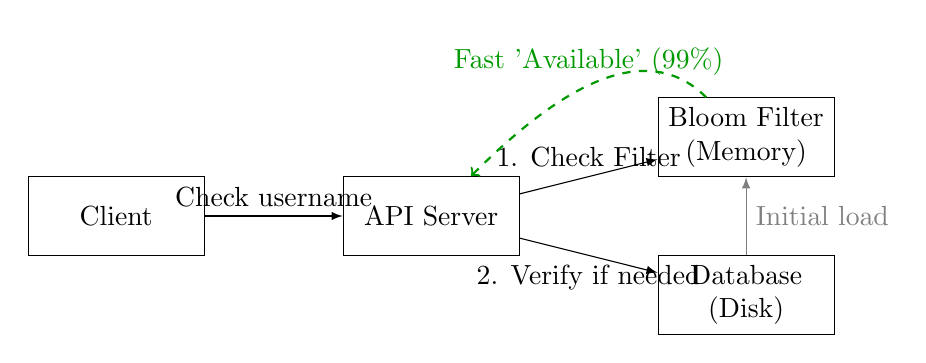
\begin{tikzpicture}[
        block/.style={rectangle, draw, text width=2cm, text centered, minimum height=1cm},
        line/.style={draw, -latex},
        cloud/.style={draw, ellipse, minimum width=2cm, minimum height=1cm}
      ]

      % Client and servers
      \node[block] (client) at (0,0) {Client};
      \node[block] (api) at (4,0) {API Server};
      \node[block] (bloom) at (8,1) {Bloom Filter (Memory)};
      \node[block] (db) at (8,-1) {Database (Disk)};

      % Connections
      \path[line] (client) -- node[above] {Check username} (api);
      \path[line] (api) -- node[above] {1. Check Filter} (bloom);
      \path[line] (api) -- node[below] {2. Verify if needed} (db);

      % Fast path annotation
      \draw[dashed, thick, green!60!black, ->] (bloom) to[out=135, in=45] node[above] {Fast 'Available' (99\%)} (api);

      % Load path
      \path[line, gray] (db) -- node[right] {Initial load} (bloom);
    \end{tikzpicture}
  \end{center}

  \begin{itemize}
    \item Bloom filter acts as a fast, efficient preliminary check.
    \item Deterministic check (DB) used only as a fallback.
    \item Massively reduces load on the expensive resource (Database).
  \end{itemize}
\end{frame}

\begin{frame}{Bloom Filters: The Theory}
  \begin{columns}
    \begin{column}{0.6\textwidth}
      \begin{itemize}
        \item Space-efficient probabilistic data structure \parencite{10.1145/362686.362692}
        \item Tests if an element is a member of a set
        \item Possible false positives, never false negatives
        \item Components:
              \begin{itemize}
                \item Bit array of $m$ bits (initially all 0)
                \item $k$ independent hash functions
              \end{itemize}
      \end{itemize}
    \end{column}
    \begin{column}{0.4\textwidth}
      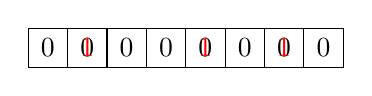
\begin{tikzpicture}[scale=0.5]
        % Draw bit array
        \foreach \i in {0,...,7} {
            \draw (\i,0) rectangle (\i+1,1);
            \node at (\i+0.5,0.5) {0};
          }

        % Show set bits
        \node at (1.5,0.5) {\textcolor{red}{1}};
        \node at (4.5,0.5) {\textcolor{red}{1}};
        \node at (6.5,0.5) {\textcolor{red}{1}};
      \end{tikzpicture}
    \end{column}
  \end{columns}
\end{frame}

\begin{frame}{Bloom Filter Operations}
  \begin{columns}
    \begin{column}{0.5\textwidth}
      \textbf{Add element:}
      \begin{enumerate}
        \item Hash element with $k$ functions
        \item Set bits at these $k$ positions to 1
      \end{enumerate}

      \textbf{Query element:}
      \begin{enumerate}
        \item Hash element with $k$ functions
        \item Check bits at these $k$ positions
        \item If \textbf{any} bit is 0: \textcolor{red}{Definitely not in set}
        \item If \textbf{all} bits are 1: \textcolor{orange}{Probably in set}
      \end{enumerate}
    \end{column}
    \begin{column}{0.5\textwidth}
      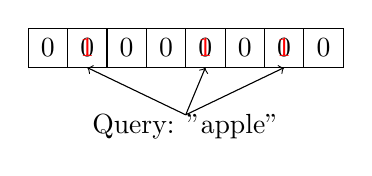
\begin{tikzpicture}[scale=0.5]
        % Draw bit array
        \foreach \i in {0,...,7} {
            \draw (\i,0) rectangle (\i+1,1);
            \node at (\i+0.5,0.5) {0};
          }

        % Update for apple
        \node at (1.5,0.5) {\textcolor{red}{1}};
        \node at (4.5,0.5) {\textcolor{red}{1}};
        \node at (6.5,0.5) {\textcolor{red}{1}};

        % Draw element and hash functions
        \node at (4,-1.5) {Query: "apple"};
        \draw[->] (4,-1.2) -- (1.5,0);
        \draw[->] (4,-1.2) -- (4.5,0);
        \draw[->] (4,-1.2) -- (6.5,0);
      \end{tikzpicture}
    \end{column}
  \end{columns}
\end{frame}

\begin{frame}{The Math Behind Bloom Filters}
  \begin{itemize}
    \item \textbf{False positive probability ($p$):}
          \begin{equation}
            p \approx \left(1 - e^{-kn/m}\right)^k
          \end{equation}\parencite{im/1109191032}

    \item \textbf{Optimal size ($m$ bits) for $n$ items, error $p$:}
          \begin{equation}
            m = -\frac{n \ln p}{(\ln 2)^2}
          \end{equation}

    \item \textbf{Optimal hash functions ($k$):}
          \begin{equation}
            k = \frac{m}{n} \ln 2 \approx 0.7 \cdot \frac{m}{n}
          \end{equation}
  \end{itemize}
\end{frame}

\begin{frame}{Time and Space Complexity}
  \begin{center}
    \begin{tabular}{l|c|c|c|c}
      \textbf{Structure} & \textbf{Space} & \textbf{Lookup} & \textbf{Insert} & \textbf{Error Type} \\
      \hline
      Hash Set           & $O(n)$         & $O(1)$ avg      & $O(1)$ avg      & None                \\
      Bloom Filter       & $O(m)$         & $O(k)$          & $O(k)$          & False Positives     \\
      Sorted List        & $O(n)$         & $O(\log n)$     & $O(n)$          & None                \\
      Trie               & $O(N)$         & $O(L)$          & $O(L)$          & None                \\
    \end{tabular}
  \end{center}

  $n$=items, $m$=bits ($m \ll n \times item\_size$), $k$=hashes, $N$=total chars, $L$=key length
\end{frame}

\begin{frame}{Bloom Filter Simulation}
  \begin{figure}[h]
    \centering
    \includegraphics[height=0.95\textheight]{./programs/bloom_filter_sim/bloom_filter_sim.png}
  \end{figure}
\end{frame}

\begin{frame}{Other Applications of Bloom Filters}
  \vspace{0.2cm}
  \begin{columns}
    \begin{column}{0.5\textwidth}
      \textbf{Web/Database:}
      \begin{itemize}
        \item Cache hit/miss optimization (e.g., CDNs)
        \item Avoid unnecessary DB lookups (like username example)
        \item Recommendation systems (seen items) \parencite{im/1109191032}
      \end{itemize}

      \textbf{Network:}
      \begin{itemize}
        \item Web crawler URL deduplication (avoid re-crawling)
        \item Network packet routing (track flows efficiently)
        \item P2P network resource discovery
      \end{itemize}
    \end{column}
    \begin{column}{0.5\textwidth}
      \textbf{Security:}
      \begin{itemize}
        \item Malware signature detection
        \item Spam filtering (known bad IPs/domains)
        \item Password breach checking (HaveIBeenPwned)
      \end{itemize}

      \textbf{Big Data:}
      \begin{itemize}
        \item Stream deduplication (unique visitors/events)
        \item Distributed data sync (approximate differences)
        \item Genomics (k-mer counting)
      \end{itemize}
    \end{column}
  \end{columns}
\end{frame}

\begin{frame}{When to Use Bloom Filters}
  Bloom filters are ideal when:

  \begin{itemize}
    \item Memory is a critical constraint (Big Data, embedded systems)
    \item False positives are acceptable (can be handled by a secondary check)
    \item False negatives are unacceptable (must find all true positives)
    \item Elements are expensive to store or compare
    \item Lookup speed is crucial (real-time systems)
    \item Deletions are not needed (or use variants like Counting Bloom Filters)
  \end{itemize}
\end{frame}